\documentclass[final]{beamer}
\mode<presentation>
{
  \usetheme{FX}
}
\graphicspath{{figures/}}

\usepackage{times}
\usepackage{amsmath,amssymb}
\usepackage[english]{babel}
\usepackage[utf8]{inputenc}
\usepackage[orientation=landscape,size=a4,scale=1.4]{beamerposter}  % e.g. custom size poster
\usepackage{listings}

  \title[MVA Project]{Object Recognition \& Graphical models : A Greedy Algorithm for Tracking a Variable Number of Objects}
  \author[Thomas]{François-Xavier Thomas}
  \institute[ENS Cachan]{MVA Master, ENS Cachan}
  \date{Jan., 5th 2012}
  \begin{document}
  \begin{frame}
    \begin{block}{\huge What is object tracking?}
      \LARGE
      \begin{itemize}
        \item An object detector returns the positions of objects on each frame, but isn't aware of time relationships
        \item Tracking is grouping together successive positions of the same object in each frame
      \end{itemize}
      \centering
      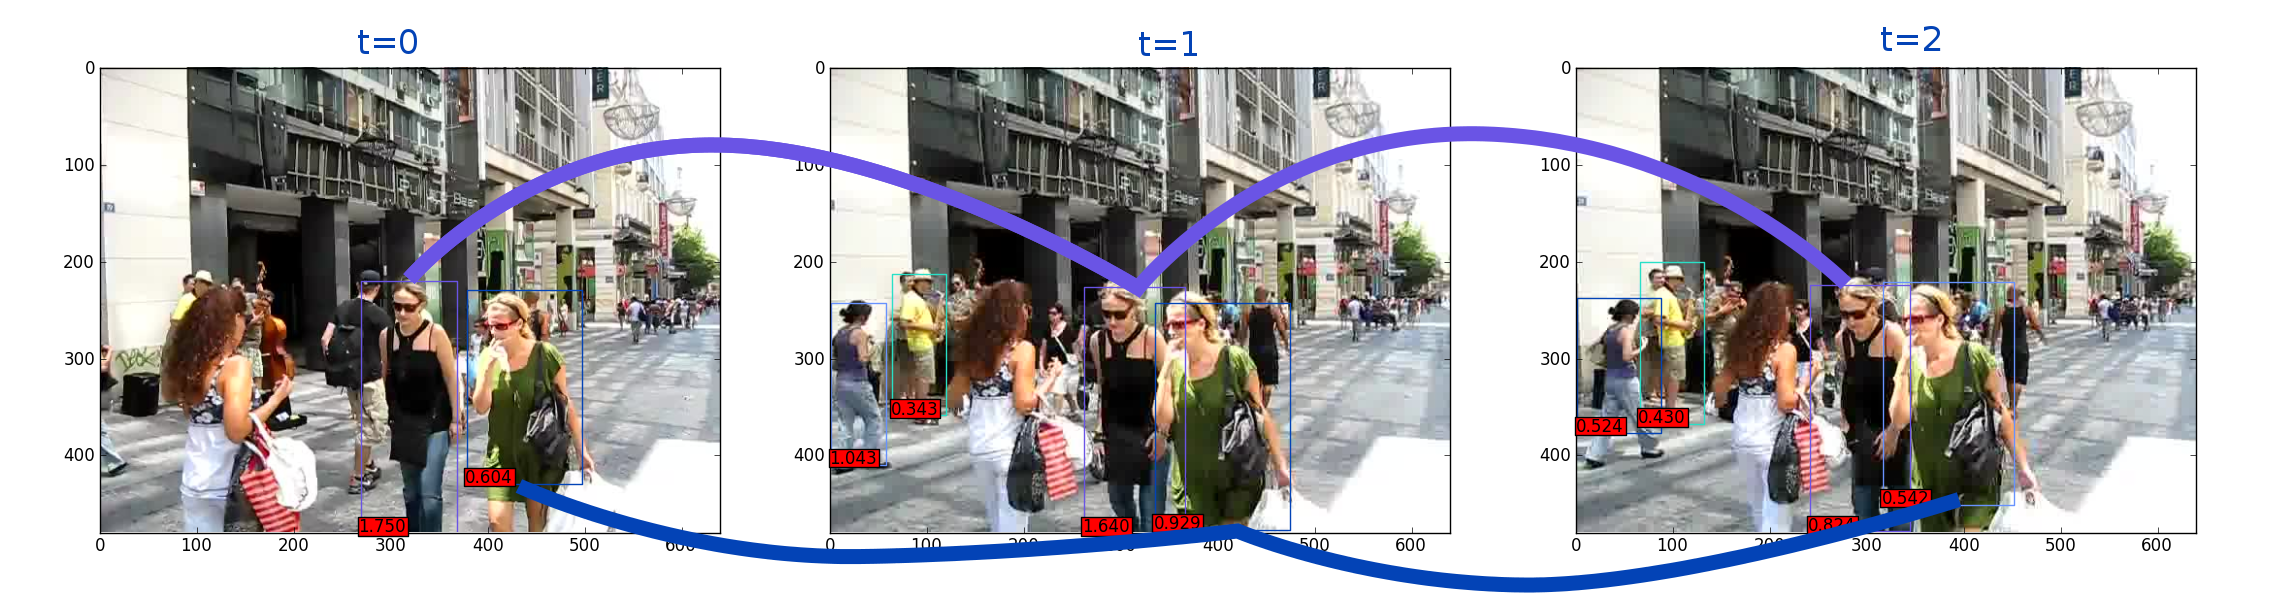
\includegraphics[width=0.95\linewidth]{figures/tracking-frames.png}
    \end{block}
  \end{frame}
  \begin{frame}
    \begin{block}{\huge Object Detection}
      \LARGE
      \begin{columns}
        \begin{column}{.30\textwidth}
          \centering
          My object detection algorithm\\
          \emph{HOG and BoW}
          \vskip5mm
          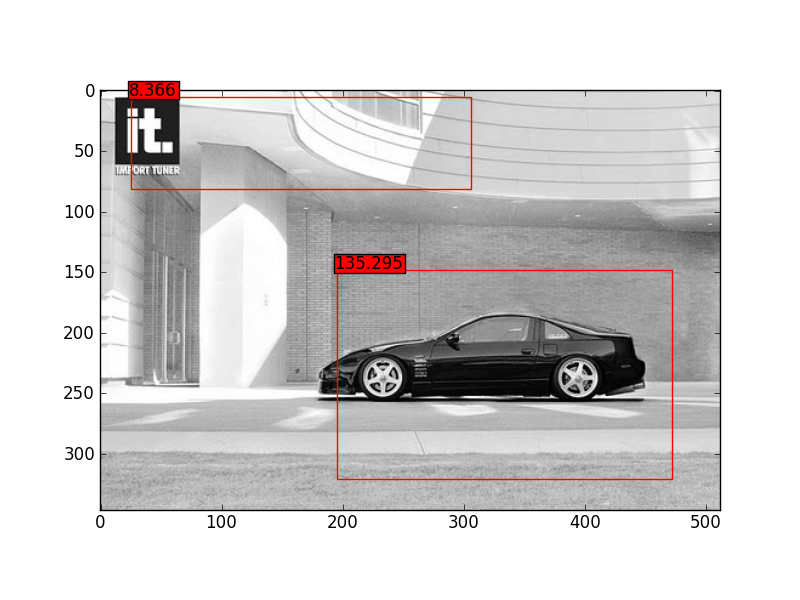
\includegraphics[width=0.95\linewidth]{figures/detection-mine.png}
        \end{column}
        \begin{column}{.30\textwidth}
          \centering
          Object detection algorithm used in the paper\\
          \emph{HOG and deformable models}
          \vskip5mm
          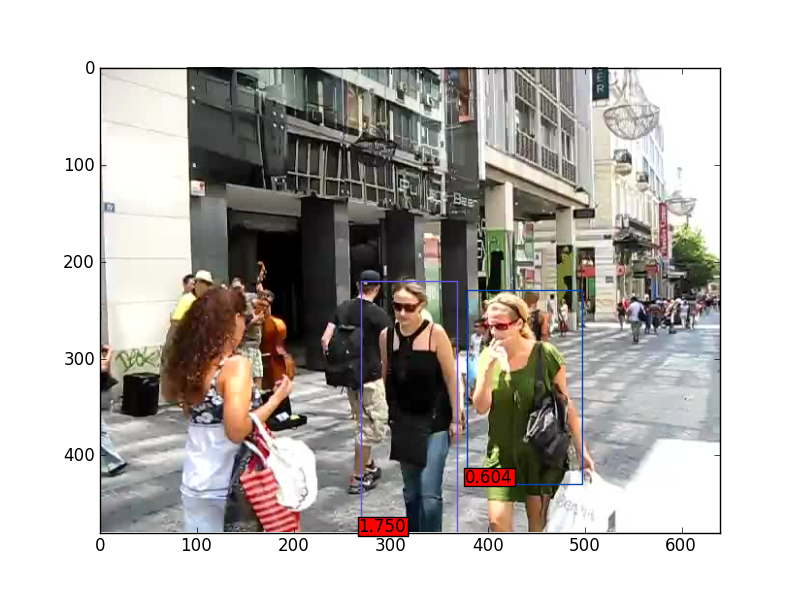
\includegraphics[width=0.95\linewidth]{figures/detection-paper.png}
        \end{column}
        \begin{column}{.30\textwidth}
          \centering
          Ground truth\\
          \emph{Selected by real people}
          \vskip5mm
          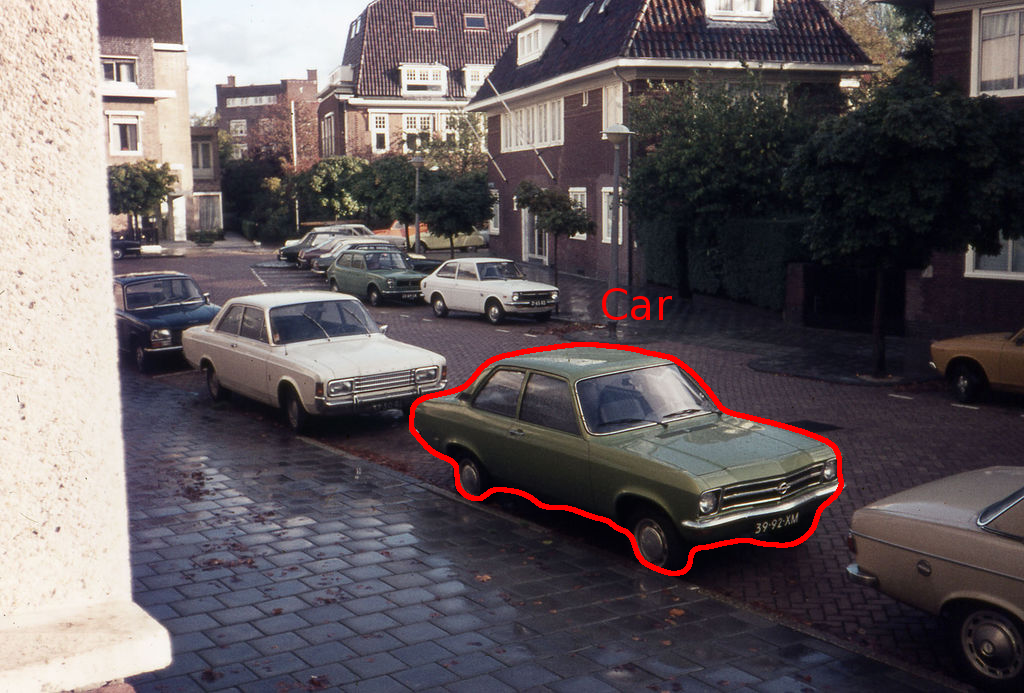
\includegraphics[width=0.95\linewidth]{figures/detection-ground.png}
        \end{column}
      \end{columns}
      \vskip5mm
      \begin{itemize}
        \item Object detection doesn't need to be very accurate for tracking.
        \item But conservative thresholds are better : they will help the algorithms decide in case of low scores in a few frames, for instance.
        \item One can use ground truths from common datasets to avoid the issue of detection
      \end{itemize}
    \end{block}
  \end{frame}
  \begin{frame}
    \begin{block}{\huge Track estimation -- Graph-based method}
      \LARGE
      \begin{columns}
        \begin{column}{.45\textwidth}
          Edge costs :
          \begin{itemize}
            \item A cost for selecting a node on the track (the more probable the
            window, the lesser the cost $c_i$ -- in red)
            
            \item A cost for creating (instantiating) a track at a specific node
            ($c_i^{\left( s \right)}$, in yellow)
            
            \item A cost for destroying a track at a specific node ($c_i^{\left( t
            \right)}$, in purple)
            
            \item A cost for transitioning between nodes ($c_{i, j}$ in blue)
          \end{itemize}
          To find the minimum cost path, one can use the \emph{Bellman-Ford} algorithm. Its complexity is roughly $\mathcal{O} \left( N^3 \right)$, with $N$ windows in state space and time.
        \end{column}
        \begin{column}{.50\textwidth}
          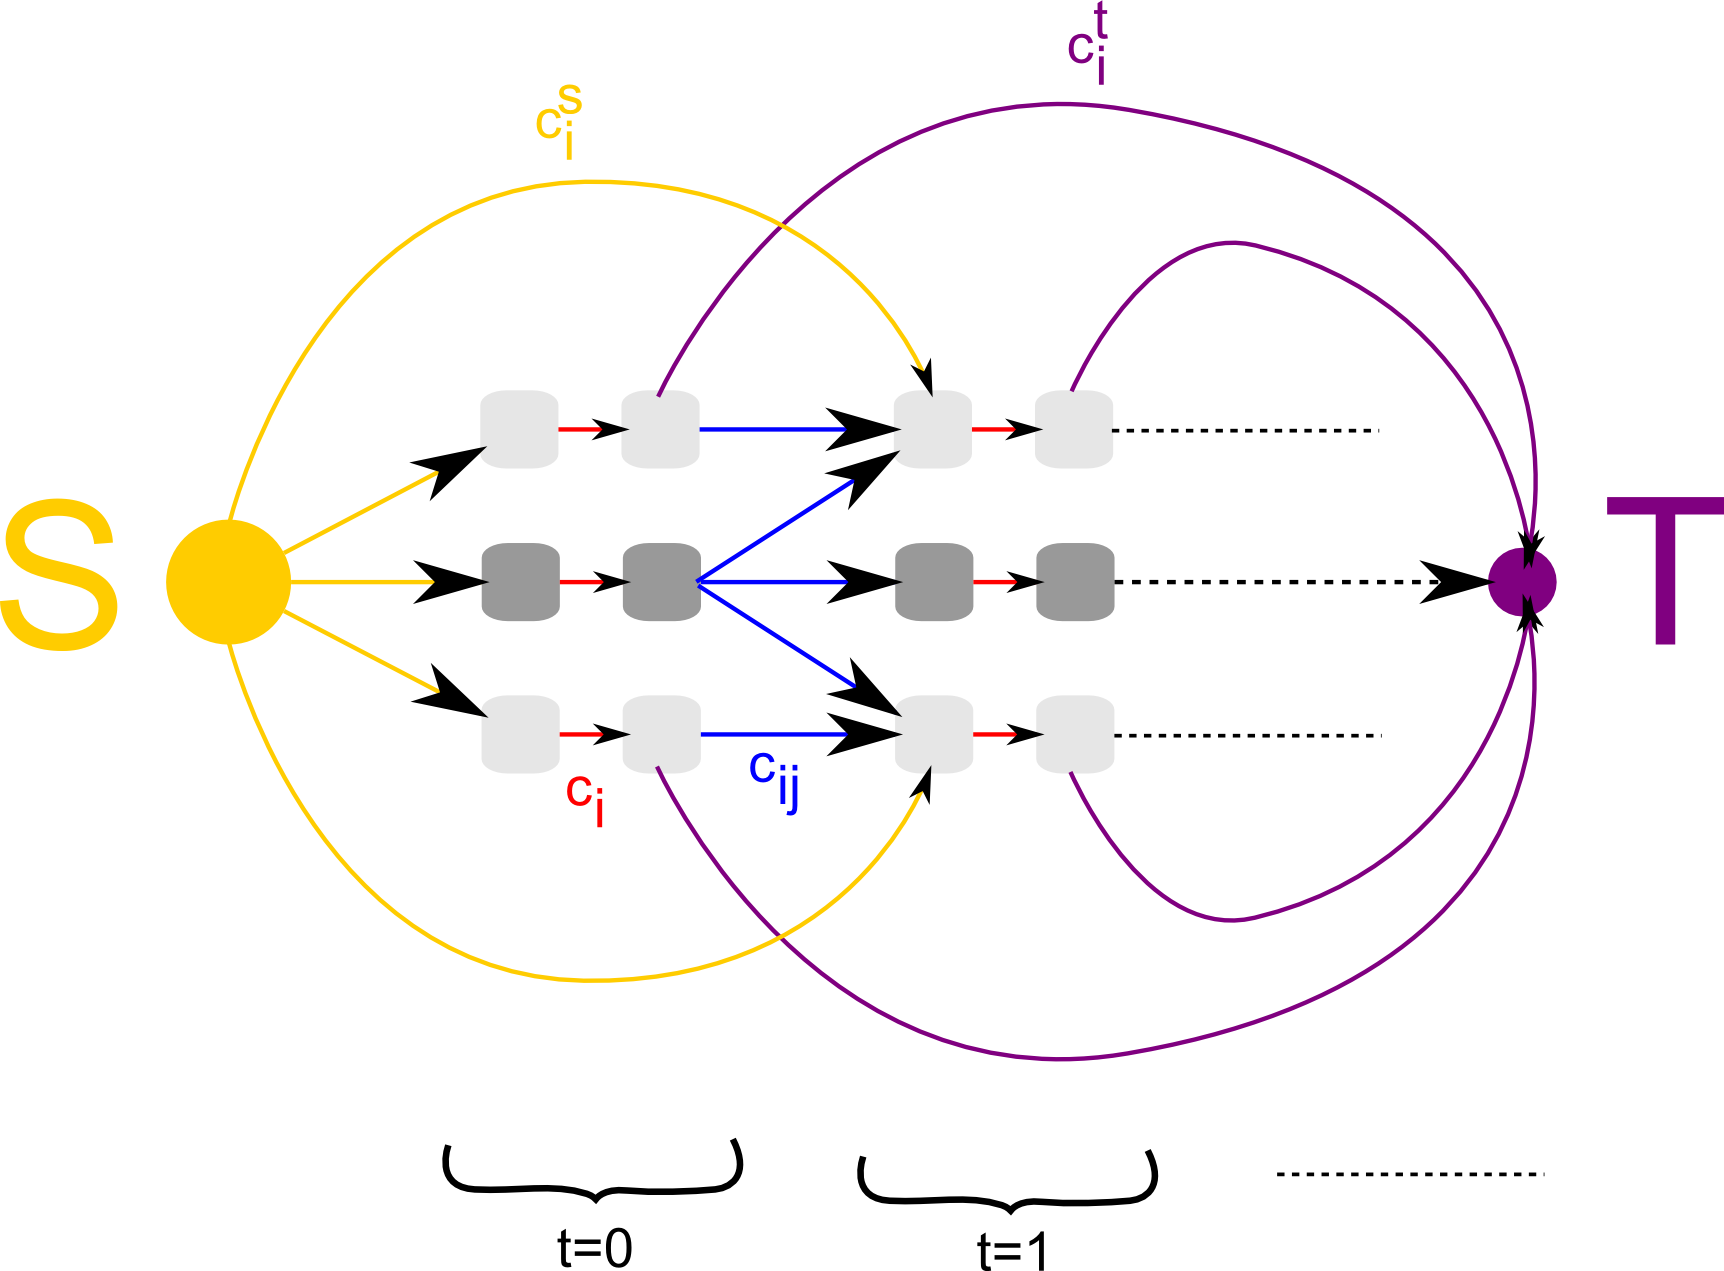
\includegraphics[width=0.95\textwidth]{figures/graph-sketch.png}
        \end{column}
      \end{columns}
    \end{block}
  \end{frame}
  \begin{frame}
    \begin{block}{\huge Track estimation -- Viterbi-based method}
      \LARGE
      The Viterbi algorithm ($y_t$ being the observed data at frame $t$, and $x$ a state) computes the probabilities of the most probable paths to state $x$ at time $t$, $V_{t,x}$ :
      \begin{itemize}
        \item For the first frame, $V_{0,x} = p\left(y_0|x \right) \times \pi_x$
        \item For the other frames, $V_{t,x} = p\left(y_t|x \right) \times \max_{z \in X_{t-1}} \left( p\left( z|x \right) \times V_{t-1,z} \right)$
        \item Store back-pointers to remember what is the parent of the last item of each best path
      \end{itemize}
      \vskip5mm

      In the paper :
      \begin{itemize}
        \item The actual $V_{t,x}$ are not computed. Instead, its authors compute a cost based on $-log V_{t,x}$ to prevent floating point errors.
        \item They also added clauses in the original Viterbi algorithm to allow track instantiation/destruction at any point in time, not just at the first and last frame.
      \end{itemize}
    \end{block}
  \end{frame}
  \begin{frame}
    \begin{block}{\huge Multiple track estimation -- Successive shortest paths}
      \LARGE
      \begin{itemize}
        \item In the Bellman-Ford-based method, the exact optimization can be computed by successively finding shortest paths on residual graphs until their total cost is greater than 0.
        \item However, we can compute an approximate solution with the Viterbi method by simply removing the previously found shortest paths and running Viterbi again until the total cost of the path is greater than 0. This solution isn't optimal, but in practice it yields good results.
      \end{itemize}
    \end{block}
    \begin{block}{\huge Improvements to the original algorithm}
      \LARGE
      \begin{itemize}
        \item In my implementation, the probability of transition between states is not uniform, but decreases when the distance between states increases. This prevents track transitions to happen between states that are fare away from each other.
        \item The similarity between state windows could also influence this probability to be able to only connect windows that look similar.
      \end{itemize}
    \end{block}
  \end{frame}
\end{document}


%%%%%%%%%%%%%%%%%%%%%%%%%%%%%%%%%%%%%%%%%%%%%%%%%%%%%%%%%%%%%%%%%%%%%%%%%%%%%%%%%%%%%%%%%%%%%%%%%%%%
%%% Local Variables: 
%%% mode: latex
%%% TeX-PDF-mode: t
